\documentclass{article}
\usepackage{graphicx}
\graphicspath{{fig/}}
\usepackage{natbib}

\title{About Table 1 in \citet{meinshausen06false}}
\author{Pierre Neuvial \& Etienne Roquain}
\begin{document}
\maketitle

Goal: elaborate on Table 1 in \cite{meinshausen06false}.  This table reports ``the  probability (in \%) of underestimating the true proportion of false discoveries (using $\alpha=0.05\%$) for some $t\in[0,1]$'' when using his proposed confidence bound ``$V(t)$'' on the number of false discoveries.

Original simulation settings as described in \cite{meinshausen06false}:
``\emph{The number of hypotheses is chosen as $m=1000$. The response variable $Y$ has a Bernoulli distribution with $p=0.5$. The predictor variable $X$ is normally distributed $X \sim \mathcal{N}(\mu,\Sigma)$ where the covariance matrix $\Sigma$ is given by $\sigma_{ii}=1$ and $\sigma_{ij}=\rho$ for $i\neq j$ and some $0\leq \rho \leq 1$. The mean is given by $\mu_i=0$ if $Y_i =0$ or $i \leq m_0$ and $i = 1$ otherwise. Test statistics are calculated under a two-sided Wilcoxon test. A total of 500 randomly chosen permutations of the response variable are used for the construction of the lower bound $S$.}''

We are interested in the influence on $\pi_0$ and $\rho$.

\section{Same settings}
Our first step was to try reproducing the results reported in the paper.  Initially we tried to use the \texttt{howmany} package to do this;  however we identified a major bug in the code, which led us to believe that this was not the code used to make this table.  Therefore (and as the code of the package was quite slow anyway), we decided to use our own code.  This code provides a faster calculation of the Wilcoxon sum rank statistic and relies on our preliminary implementation of joint FWER control. 


The results are reported in Table~\ref{tab:400-3} for $m_1=400$ ($\pi_0=0.6$) and Table~\ref{tab:10-3} for $m_1=10$ ($\pi_0=0.6$).
% latex table generated in R 3.1.0 by xtable 1.7-1 package
% Fri Jan 31 20:42:14 2014
\begin{table}[ht]
\centering
\begin{tabular}{llll}
  \hline
 & $n=20$ & $n=60$ & $n=100$ \\ 
  \hline
$\rho=0$ & $0.7\pm0.5$ & $1.1\pm0.7$ & $0.6\pm0.5$ \\ 
  $\rho=0.2$ & $2\pm0.9$ & $2.9\pm1.1$ & $1.4\pm0.7$ \\ 
  $\rho=0.4$ & $3.4\pm1.1$ & $2.7\pm1$ & $2.4\pm1$ \\ 
   \hline
\end{tabular}
\caption{$m_1=400$.} 
\label{tab:400-3}
\end{table}

\begin{table}[ht]
\centering
\begin{tabular}{llll}
  \hline
 & $n=20$ & $n=60$ & $n=100$ \\ 
  \hline
$\rho=0$ & $3.3\pm1.1$ & $3.5\pm1.2$ & $3.7\pm1.2$ \\ 
  $\rho=0.2$ & $3.5\pm1.2$ & $4.4\pm1.3$ & $3.4\pm1.1$ \\ 
  $\rho=0.4$ & $4.8\pm1.4$ & $4.1\pm1.3$ & $4.6\pm1.3$ \\ 
   \hline
\end{tabular}
\caption{$m_1=10$.} 
\label{tab:10-3}
\end{table}
Note that we provide an estimate of (twice) the standard error $\hat{\sigma}$ of the estimate $\hat{p}$ of the probability: $\hat{\sigma} =\sqrt{\hat{p}(1-\hat{p})}/\sqrt{B}$, where $B$ is the number of simulations.  Here $B=1,000$ (it was $500$ in the paper). 

Because $\hat{\sigma}$ is fairly large it is hard to conclude much from these tables, except that the estimates in \cite[Table 1]{meinshausen06false} are consistent with the one we obtained. 

\section{Increasing the number of experiments}
In order to get tighter estimates we replicated the experiment $B=10,000$ times instead of $1,000$. Note that this would have been quite long using the implementation of the \texttt{howmany} package (probably in the order of months of CPU for each estimate).  With our implementation each estimate is obtained in a matter of hours (using plain R code). 

% latex table generated in R 3.1.0 by xtable 1.7-1 package
% Sun Feb  2 21:40:50 2014
\begin{table}[ht]
\centering
\begin{tabular}{llll}
  \hline
 & $n=20$ & $n=60$ & $n=100$ \\ 
  \hline
$\rho=0$ & $4.18\pm0.4$ & $3.78\pm0.4$ & $4.33\pm0.4$ \\ 
  $\rho=0.2$ & $4.5\pm0.4$ & $4.2\pm0.4$ & $3.66\pm0.4$ \\ 
  $\rho=0.4$ & $4.75\pm0.4$ & $4.56\pm0.4$ & $4.48\pm0.4$ \\ 
   \hline
\end{tabular}
\caption{$m_1=10$, $B=10,000$.} 
\label{tab:10-4}
\end{table}

% latex table generated in R 3.1.0 by xtable 1.7-1 package
% Sun Feb  2 21:41:38 2014
\begin{table}[ht]
\centering
\begin{tabular}{llll}
  \hline
 & $n=20$ & $n=60$ & $n=100$ \\ 
  \hline
$\rho=0$ & $0.59\pm0.2$ & $0.59\pm0.2$ & $0.52\pm0.1$ \\ 
  $\rho=0.2$ & $1.65\pm0.3$ & $1.76\pm0.3$ & $1.78\pm0.3$ \\ 
  $\rho=0.4$ & $2.62\pm0.3$ & $2.69\pm0.3$ & $2.94\pm0.3$ \\ 
   \hline
\end{tabular}
\caption{$m_1=400$, $B=10,000$.} 
\label{tab:400-4}
\end{table}
Under the sparse scenario of Table \ref{tab:10-4}, the obtained control is fairly tight across the range of parameter values. Under the non-sparse scenario of Table \ref{tab:400-4}, the bound is quite conservative in the independent setting ($\rho=0$); it becomes less conservative as $\rho$ increases.

Our interpretation is that this is due to a problem of ``bad $\mathcal{H}_0$".  This suggests that it could be interesting to design a step-down procedure based on the current single-step one.   However, we have to note that the configuration chosen by \cite{meinshausen06false} is essentially Dirac-Uniform, as illustrated by Figure \ref{fig:du}.
\begin{figure}
  \centering
  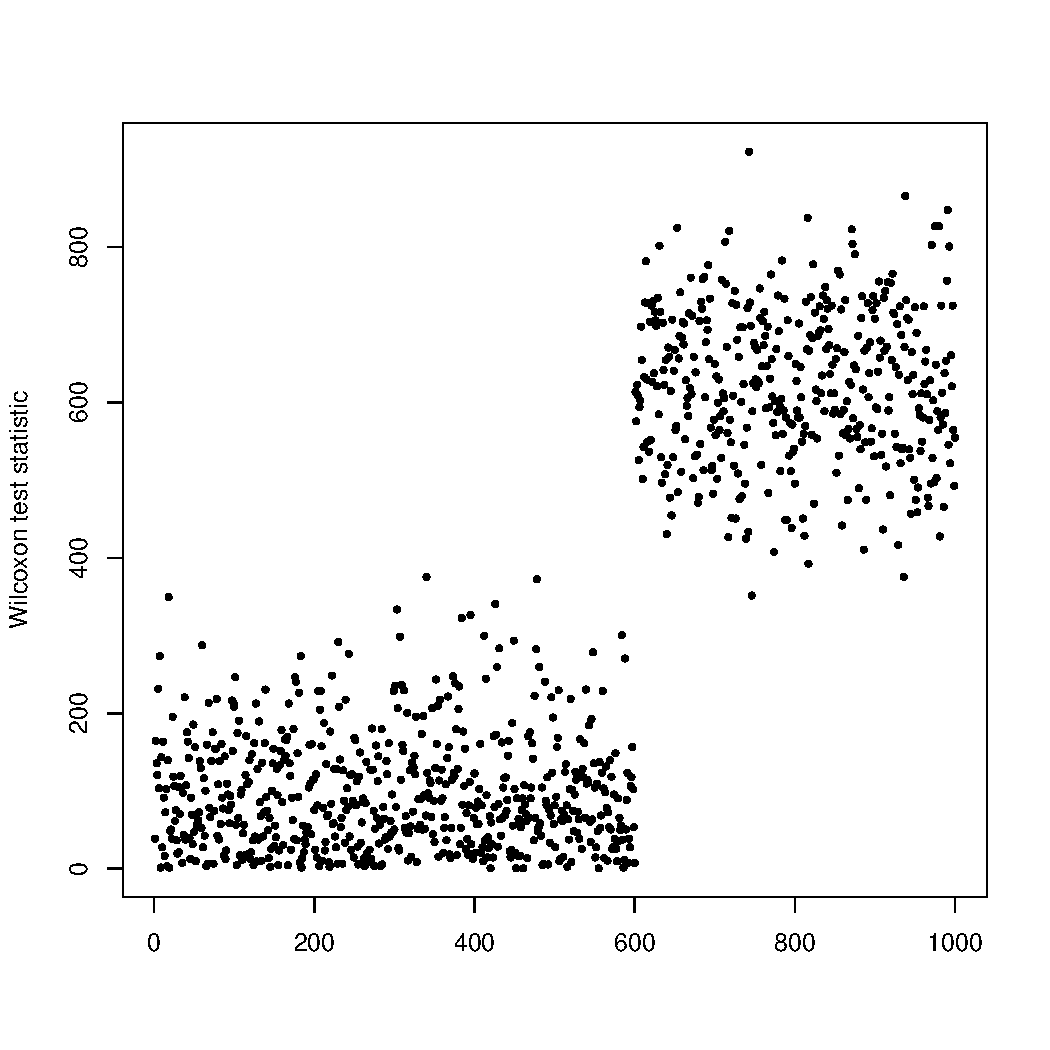
\includegraphics[scale=0.45]{DU}
  \caption{$m=1000$ Wilcoxon test statistics in one experiment using the settings of \cite{meinshausen06false} with $\pi_0=0.6$. Guess which are the true alternatives.}
  \label{fig:du}
\end{figure}



\section{Under the global null}
For completeness, we report in Table \ref{tab:0-4} the results obtained when $m_1=0$ ($\pi_0=1$):
% latex table generated in R 3.1.0 by xtable 1.7-1 package
% Sun Feb  2 21:37:40 2014
\begin{table}[ht]
\centering
\begin{tabular}{llll}
  \hline
 & $n=20$ & $n=60$ & $n=100$ \\ 
  \hline
$\rho=0$ & $6.39\pm0.5$ & $6.58\pm0.5$ & $6.88\pm0.5$ \\ 
  $\rho=0.2$ & $5.33\pm0.4$ & $5.31\pm0.4$ & $5.68\pm0.5$ \\ 
  $\rho=0.4$ & $4.93\pm0.4$ & $5.37\pm0.5$ & $5.13\pm0.4$ \\ 
   \hline
\end{tabular}
\caption{$m_1=0$, $B=10,000$.} 
\label{tab:0-4}
\end{table}

\bibliographystyle{plainnat}
\bibliography{mein}
\end{document}
